% Template for ICIP-2009 paper; to be used with:
%          spconf.sty  - ICASSP/ICIP LaTeX style file, and
%          IEEEbib.bst - IEEE bibliography style file.
% --------------------------------------------------------------------------
\documentclass{article}
\usepackage{spconf,amsmath,epsfig}

% Example definitions.
% --------------------
\def\x{{\mathbf x}}
\def\L{{\cal L}}

% Title.
% ------
\title{PEDESTRIAN DETECTION USING HAAR-LIKE FEATURES}
%
% Single address.
% ---------------
\name{Tim Besard, Ruben Schollaert, Dimitri Roose, Sebastiaan Labijn}
%\thanks{Thanks to University College Ghent for funding.}
\address{University College Ghent\\Applied Engineering\\Campus Schoonmeersen, Valentin Vaerwyckweg 1, 9000 Gent}


\begin{document}
%\ninept
%
\maketitle
%
\begin{abstract}
%The abstract should appear at the top of the left-hand column of text, about
%0.5 inch (12 mm) below the title area and no more than 3.125 inches (80 mm) in
%length.  Leave a 0.5 inch (12 mm) space between the end of the abstract and the
%beginning of the main text.  The abstract should contain about 100 to 150
%words, and should be identical to the abstract text submitted electronically
%along with the paper cover sheet.  All manuscripts must be in English, printed
%in black ink.
% Begin abstract
In this paper a solution for pedestrian detection is described using Haar-like features. It is being developed to be used in a tram collision advoidance project. 
\end{abstract}
%
\begin{keywords}
Pedestrian Detection, Haar-like Features, AdaBoost Classification
\end{keywords}
%
\section{Introduction}
\label{sec:intro}

Object detection is a very important element in computer vision areas. The goal is to find a predefined object in a set of images or video frames. This task can be fulfilled using template matching techniques extracting certain image features such as edges, color regions, textures and contours.
\par
Alas for complex objects such as pedestrians these features are hard to find due the great variety of instances of these pedestrians. This huge variety is caused by the following major problems~\cite{monteiro2006vision}:

\begin{itemize}
\item The size, color and style of pedestrian clothing are very diverse.
\item Pedestrians are nong-rigid bodies. Their shape and size differ greatly and therefore they are more complex then rigid objects.
\item Not only the pedestrians are part of the problem, but the background too. It can cause cluttering or can be mistaken for pedestrians due to its composition.
\item Illumination and weather conditions can lower the distinction between background and pedestrian.
\item Also the lack in motion due the slow speed of pedestrians hardens the possibility for them to be detected.
\end{itemize}

Instead of using the template matching approach, another possible method has been described by Viola and Jones~\cite{viola2001rapid}.

\section{How it works}
This approach uses statistical models, so called classifiers. These are created by extensive training using a pool of test images. These pools consists of positive and negative samples, respectively images that contain pedestrians and images that don't. 
From these sample images features will be extracted and the features which classify that pedestrians are selected. These are the so called Haar-like features. The general flow of this process is shown in Figure~\ref{fig:flowchart}.

\begin{figure}[H]
	\centering
	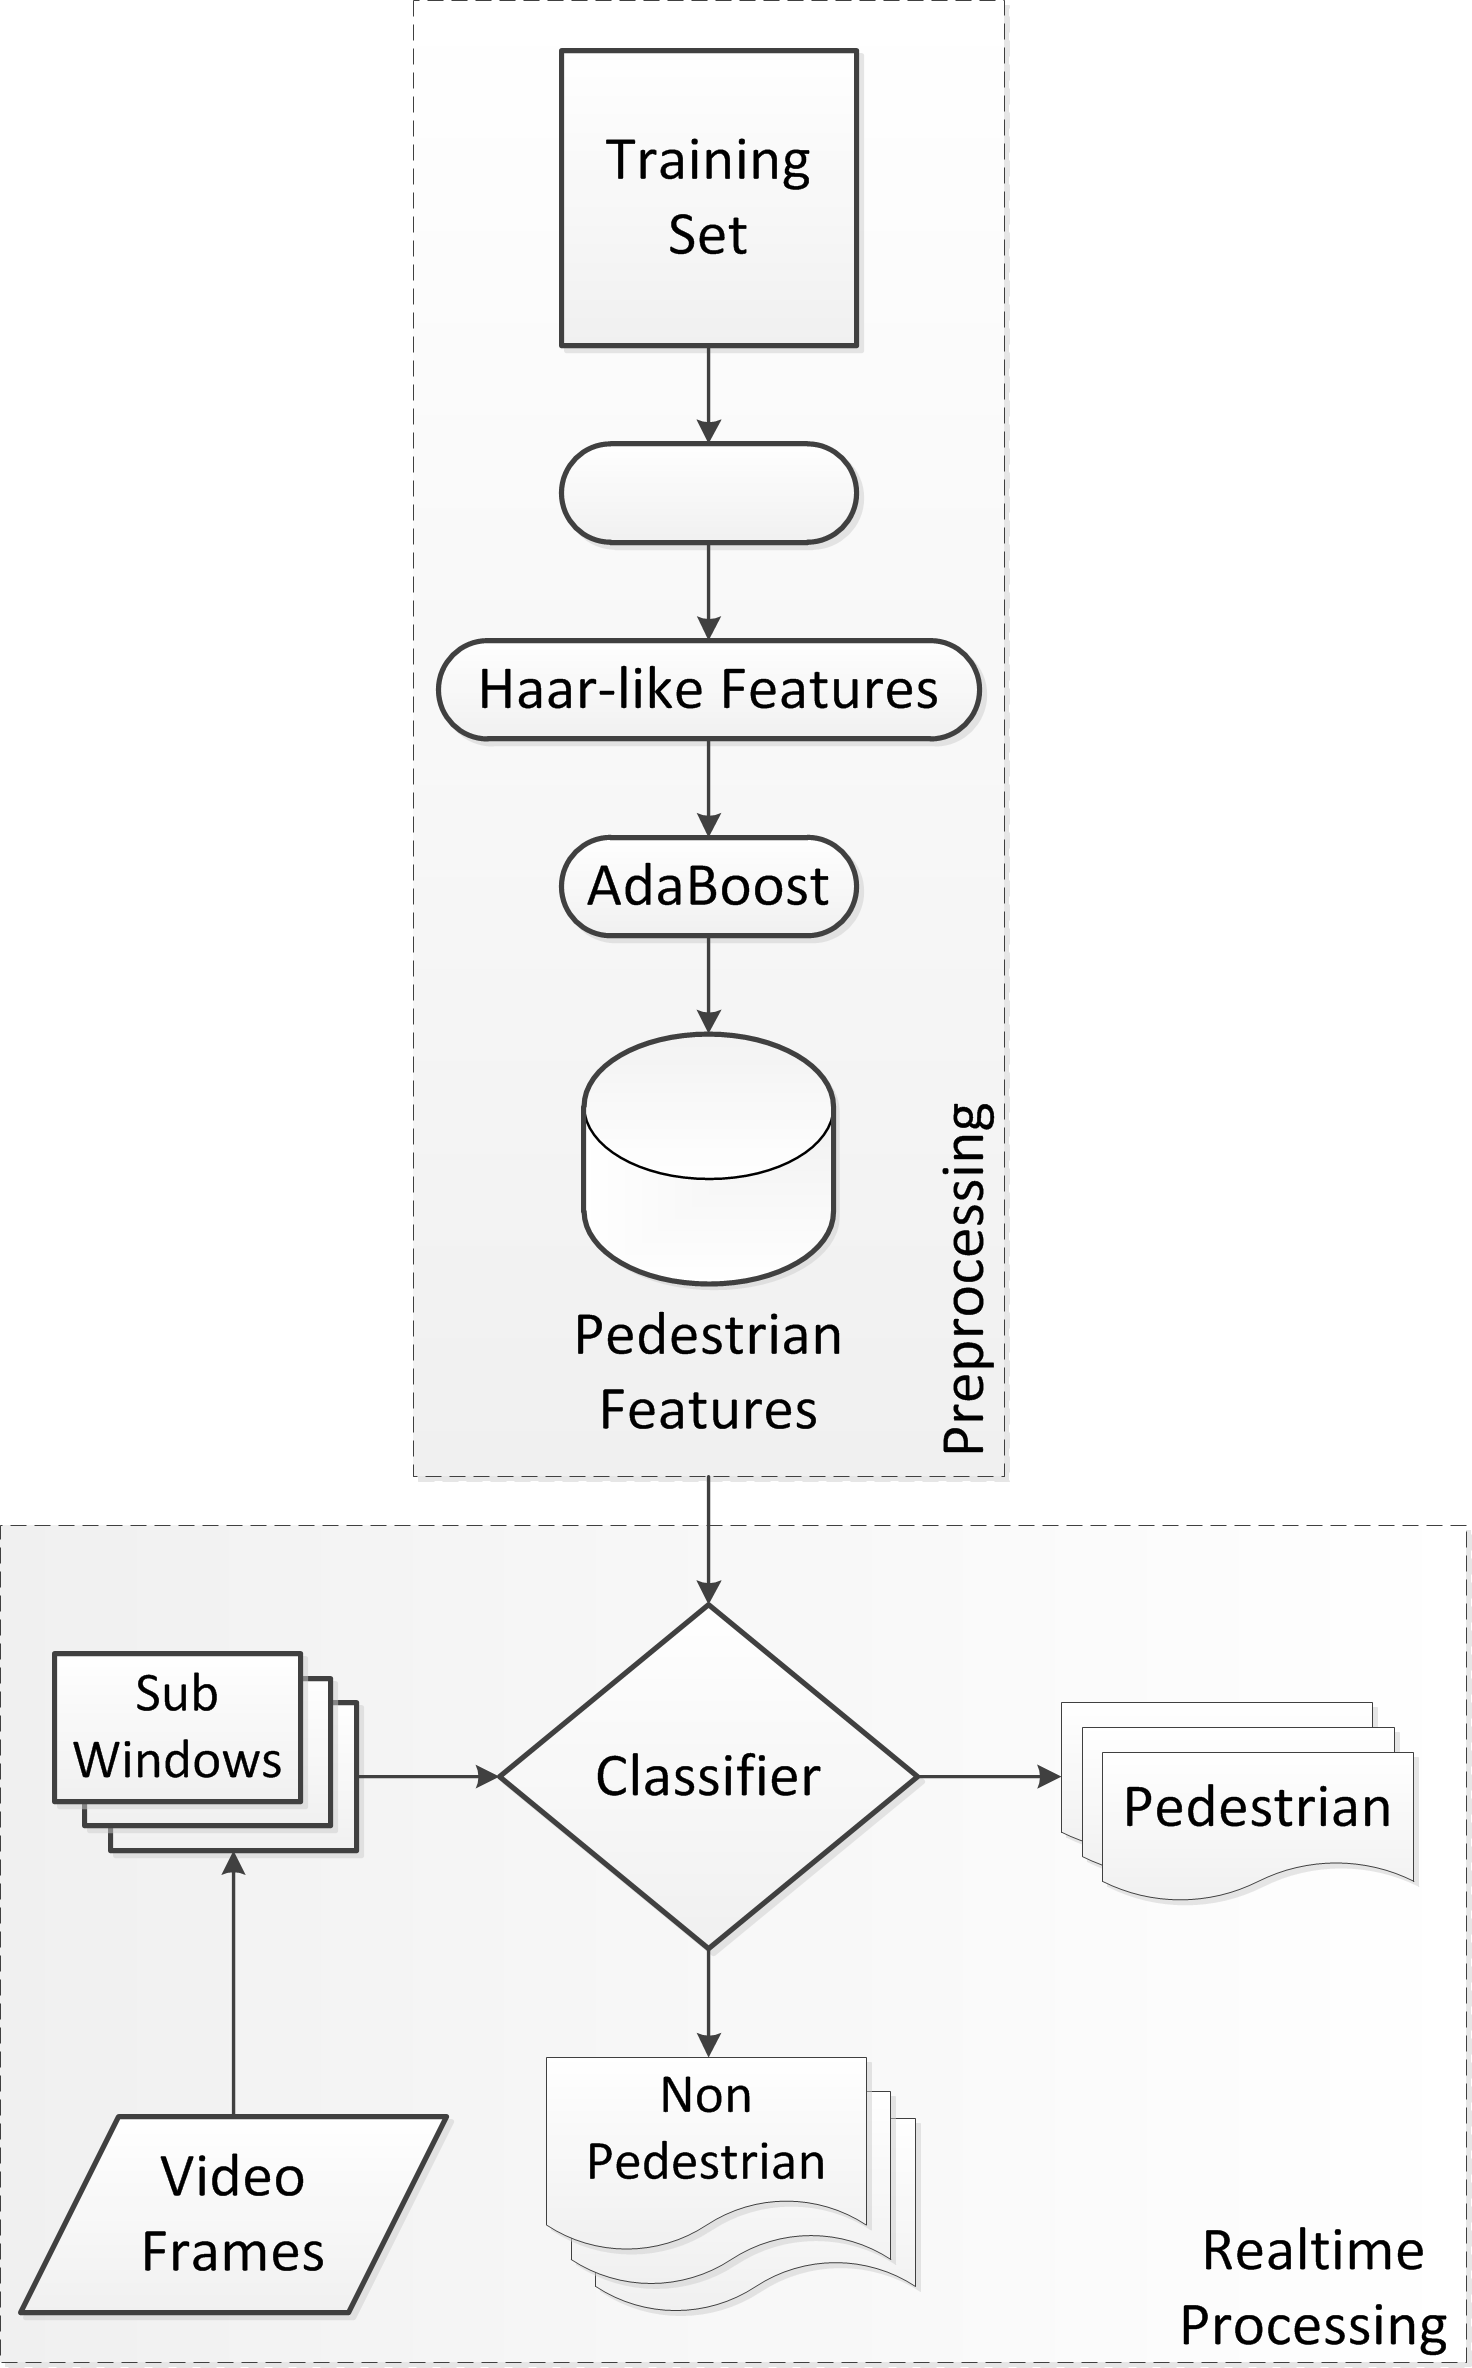
\includegraphics[scale=0.5]{HaarTrainingFlowChart.png}
	\caption{Flowchart for detecting pedestrians.}
	\label{fig:flowchart}
\end{figure}

%The Haar-like features (so called because they are computed
%similarly to the coefficients of Haar wavelet trans-
%forms) and a large set of very simple “weak”
%classifiers, that use a single feature to classify
%the image as pedestrian or non-pedestrian, were
%used to extract the features characteristics of the
%pedestrians.
%
%and extended by Lienhart et al. [1,2]. In one image
%sub-window, the total number of Haar-like fea-
%tures is very large, far larger than the number of
%pixels. In order to ensure a fast classification, the
%learning process must exclude a large majority of
%the available features, and focus on a small set of
%critical features. A variant of AdaBoost [4] is used
%for making those features selection (see Figure 1).
%Training Set
%Normalization
%A similar methodology combining Haar-like fea-
%tures and the AdaBoost algorithm, proposed by
%Viola et. al. to detect faces, is proposed here to
%detect pedestrians on the road.

% TODO Per sectie beetje uitleg geven.
\section{Haar-like features}

A Haar-like feature is represented by a template, its coordinate relative to the sub window and his size.
The template, a shape, is composed of two or three rectangles joined together. Each of these rectangles is colored black or white. Three of these Haar-like features are displayed in Figure~\ref{fig:features}. These rectangles can be turned horizontal, vertical or even  diagonal, an extension proposed in~\cite{lienhart2002extended}.

\begin{figure}[H]
	\centering
	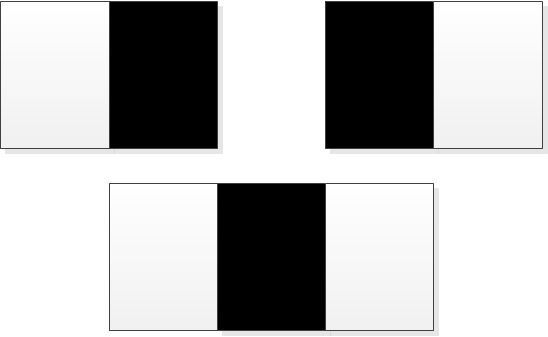
\includegraphics[scale=0.6]{Features.png}
	\caption{Prototypes of Haar-like features.}
	\label{fig:features}
\end{figure}

\par
Foreach feature a value is calculated for each position in the search sub window. These values sum up the pixel intensities in these regions and calculates the difference between them. This difference is then used to check wether the feature resembles with this position on the sub window.

\par
A subwindow of an image contains a far larger amount of features than pixels. Therefore a mechanism is needed to select the most valuable ones.

\section{AdaBoost}

Once a machine learning system has a training set of positive and negative samples and a feature set it can be invoked to fulfill the training of the classifier. Viola and Jones~\cite{viola2001rapid} used a variant of AdaBoost to both select a small set of features and to train the classifier. In its original form, the AdaBoost learning algorithm is used to boost the classification performance of a simple  learning algorithm.

\par
Although each feature can be computed very efficiently, the computation of the complete feature set is unfeasible.

\par
Building the boosted classifiers takes the most time because it requires a lot of training data and iterations in the AdaBoost algorithm. Once these classifiers are built, the detection is capable of processing images extremely rapidly and achieving high detection rates~\cite{viola2001rapid}.

\section{Training a cascade of classifiers}

A cascade of classifiers consists of multiple weaker classifiers. The simpler classifiers go first, they will then reject the majority of the negative matches. When a window passes these simpler classifiers, more complex ones are used. This causes a lower false positive rate.

Each round of this cascade was trained using AdaBoost. Adaboost is an algorithm for constructing a strong classifier as a linear combination of simple weak classifiers.

To have a highly efficient outcome a goal is set at the beginning, this goal contains the number of false positives and the detection rate. After this goal is set new rounds with new weak classifiers are added to the cascade. After every round the new cascade of classifiers is tested on a validation set. If the goal is not yet reached, new rounds are added over and over again.

To create a successful cascade of classifiers a lot of samples are required. These samples contain images from pedestrians in all possible poses, sizes and with different clothing. A large number of samples (1000+) are required for a good detection rate.  Besides these positive pedestrian images we also require negative samples. The negative samples can just be the positive images backgrounds.

A pedestrian detection cascade file, as delivered with OpenCV, contains 30 rounds. Each round contains 40 features. 





\section{OpenCV Haartraining}
To create and test the cascade of boosted classifiers based on Haar-like features we are using OpenCV \cite{opencv_library}. OpenCV provides us programs that we can use to create our own classifiers.

\subsection{Create samples}
Before we can start creating samples we need positive images, these are images which contain pedestrians without much variations in the illumination, if there are too many variations the resulting detector will not work well.
Besides the positive images we also need negative images and testing images. The testing images are images combined with the location of the pedestrians. We used the CBCL PEDESTRIAN DATABASE \#1 from MIT which contains 924 images.
From one image we can create several samples by using distortion, we can use the createsamples program delivered by OpenCV for this. For example 

createsamples -img image.png -num 10 -bg negatives.dat -vec samples.vec -w 64 -h 128

will generate 10 samples out of one image.
The file 'negatives.dat' is a file containing a list of the negative images used.

For the test images we need to create a file which includes the location of the pedestrian in each image. This file will just hold the x and y coordinates in combination with the height and width of the pedestrian.
After these steps we can start creating the testing samples, these are created as follows:

createsamples -img image.png -num 10 -bg negatives.dat -info test.dat -maxxangle 0.6 -maxyangle 0 -maxzangle 0.3 -maxidev 100 -bgcolor 0 -bgthresh 0

This wil generate cropped pedestrians placed on top of negative samples as output. A description file with the coordinates of the cropped pedestrian in the new image will also be available.




\subsection{Train}

To train our classifier we can use the haartraining utility. The following training takes about four days.

haartraining -data haarcascade -vec samples.vec -bg negatives.dat -nstages 20 -nsplits 2 -npos 5000 -nneg 2500 -w 20 -h 80 -nonsym -mem 512 -mode ALL

We use the '-nonsym' parameter because people don't have a symmetric body structure in all poses. If we would be making classifiers for a symmetric object we would use the default, so only half of the image will be processed  thus speeding up the training. We also specified the '-mode ALL', this means the haartraining will look for all Haar-like features, default will only look for upright features.
Increasing the number of stages (-nstages 20) will not necessarily produce a better result. If the default threshold of minimum 99.5\% hitrate or the maximum false alarm of 50\% is reached, the training will stop.
When the training is finished, OpenCV will generate an XML outputfile.

\subsection{Test}
OpenCV also has a program to test the performance of the generated classifiers. This program is called 'performance'. Testing the XML can be done like this:
performance -data haarcascade.xml -info tests.dat -ni
The tests.dat file contains a list of testing images and the 'ni' parameter is used so the performance-utility will not output any detection images.
The performance-utility will then output the number of correct detections, the number of missed or false negatives and the number of false positives.

\section{Experimental results}

\section{Conclusion}



\bibliographystyle{IEEEbib}
\bibliography{bibliografie}

\end{document}
